\documentclass[a4paper,twocolumn,11pt]{article}
\usepackage[letterpaper,scale=0.875,right=1.3cm,top=2cm]{geometry} % Márgenes y demás
\usepackage{multicol}
%%%%%%%% TABERLLE
\usepackage[table]{xcolor} % Pacchetto per la gestione dei colori nelle tabelle
%%%%%%%% CODICE

\usepackage{listings}
\usepackage{moresize}
\lstset{showstringspaces=false} %remove space simbol
\definecolor{codegray}{rgb}{0.95,0.95,0.95}
% Definizione dei colori per i tag HTML
\definecolor{tagblue}{rgb}{0.3,0.6,0.8}
\definecolor{attrgreen}{rgb}{0.0,0.4,0.0}
\definecolor{valueorange}{rgb}{0.8,0.4,0.0} 



\usepackage[utf8]{inputenc}
\usepackage{pxfonts}
\usepackage{wasysym} % symbols
\usepackage{abstract}
\usepackage{parskip}
\usepackage{microtype}
\usepackage{verbatim}   
\usepackage[hyperindex=false,breaklinks=false,colorlinks=false,linkcolor=false]{hyperref}
\usepackage{graphicx}
%\def\sym##1{\ifmmode^{##1}\else\(^{##1}\)\fi}
\usepackage{titlesec}
\usepackage{xcolor}
%no quitar nada
\hypersetup{
    colorlinks=true,
    linkcolor=carnelian, % Color para enlaces internos
    urlcolor=carnelian,   % Color para enlaces URL
    citecolor=carnelian, % Color para citas bibliográficas
}
\usepackage{float}
\usepackage{graphicx}
\usepackage{blindtext}% only for dummy text
\usepackage{fancyhdr}
\usepackage{titling}
\usepackage{caption}
\usepackage{dcolumn}

\captionsetup[table]{
  position=above,
  justification=raggedright,
  labelsep=newline, % <<< label and text on different lines
  singlelinecheck=false % <<< raggadright also when the caption is shorter
                        % than a single line
}
\usepackage[document]{ragged2e}
\usepackage[affil-sl]{authblk} 
\usepackage{mathptmx}  %Times new Roman


%$$$$$$$$$$$$$$$$$$$$$$$$$$$$$$$$$$$$$$$$$$$$
\usepackage{orcidlink}







\setlength{\columnsep}{1cm}
\renewcommand{\refname}{REFERENCES}
\renewcommand{\figurename}{Fig.}


% Keywords command
\providecommand{\keywordsSpan}[1]
{
  \small	
  \textbf{\textit{Palabras Clave:}} #1
}

\providecommand{\keywordsEng}[1]
{
  \small	
  \textbf{\textit{Keywords:}} #1
}





\pagestyle{fancyplain}% <- pagestyle fancyplain
\fancyfoot[C]{}
\renewcommand\plainheadrulewidth{.4pt}% headrule on plain pages
%\fancyhf{}
\fancyhead[C]{Proposal - CSP violation due to the SOP}
\rhead{}
\lhead{}
\rfoot{}



\definecolor{carnelian}{rgb}{0.7, 0.1, 0}

%%%%%%%% FORMATO DE LAS SECCIONES Y SUBSECCIONES %%%%%
\titleformat*{\section}{\fontsize{11}{1}\bfseries\color{carnelian}}


\titleformat*{\subsection}{\fontsize{11}{1}\bfseries\color{carnelian}\itshape}


\titlespacing*{\section}
{0pt}{1cm}{0.2cm}

\titlespacing*{\subsection}
{0pt}{1cm}{0.2cm}




 
\makeatletter
\long\def\@makecaption#1#2{
\vskip\abovecaptionskip
\sbox\@tempboxa{#1. #2}
\ifdim \wd\@tempboxa >\hsize
#1. #2\par
\else
\global \@minipagefalse
\hb@xt@\hsize{\hfil\box\@tempboxa\hfil}
\fi
\vskip\belowcaptionskip}
\makeatother


\fancypagestyle{plain}% Para la primera p\´agina
{%
\fancyhf{}
\renewcommand{\headrulewidth}{0.5pt}
\renewcommand{\footrulewidth}{0pt}
\fancyheadoffset[LO]{-0.42\textwidth}
\fancyhead[RO]{
\includegraphics[scale=0.25]{Figuras/unimol-universita-molise-campobasso.png} } 
\fancyhead[LO]{Anno Accademico 2022 - 2023\\ \emph{Networking security and software security}}
\fancyfoot[CO]{\footnotesize{\thepage}}
}
\fancyfoot[CO]{\footnotesize{\thepage}}


\usepackage{balance}
\usepackage{flushend}
\newcommand{\balancecolumns}{%
  \vfill\eject
  \global\@colht = \textheight
  \global\ht\@cclv = \textheight}
    

%%%%%%%%%%%%%%%%%%%%%%%%%%%%%%%%%%

\date{}  %%Llama el archivo de los estilos



%%%%%%%%%%%%%%%%%%%%%%%%%%%%%%%%%%%%%%%%%% TITOLO %%%%%%%%%%%%%%%%%%%%
{\title{
\vspace*{2cm}
\huge { CSP violation due to the SOP\\[0.4cm]
\large{\textcolor{carnelian}{\emph{Proposal}}}
\\[0.1cm]}}}

%%%%%%%%%%%%%%%%%%%%%%%%%%%%%%%%%%%%%%%%%%%% AUTORI %%%%%%%%%%%%%%%%%%%%%%%%%%%%%%%%%%%%%%%%%%%%%%
\author[1]{\fontsize{10pt}{10pt}\selectfont \textbf{Andrea D'Aguanno}}
%\author[2]{\textbf{Author 2} \orcidlink{0000-0000-0000-0000}}
%\author[1,3]{\textbf{Author 3}\orcidlink{0000-0000-0000-0000}}
\affil[1]{
\fontsize{8pt}{8pt}\selectfont Matricola n. 172359}
\fontsize{8}{8}
%\affil[2]{Affiliation of Corresponding Author 2}
%\affil[3]{Affiliation of Corresponding Author 3 \vspace{0.2cm}} 
%\affil[*]{\texttt{$^{*}$Correo autor@correspondencia.com}}

%%%%%%%%%%%%%%%%%%%%%%%%%%%%%%%%% INIZIO DEL DOCUMENTO %%%%%%%%%%%%%%%%%%%%%%%%%%%%%%%%%%%%%%%%%%%%%%
\begin{document}

\twocolumn
[
\begin{@twocolumnfalse}
\maketitle
%\begin{flushleft}
%    \textbf{Received:} XXXXX\\
%    \textbf{Accepted:} XXXXX\\
%    \textbf{How to cite:} XXXXX\\
%    \textbf{DOI:} XXXXX\\
%\end{flushleft}

\vspace*{0.3cm}
\vspace{0.2cm}
\hspace*{0.7cm}

%%%%%%%%%%%%%%%%%%%%%%%%%%--> Abstract
\renewcommand{\abstractname}{\textcolor{carnelian}{ABSTRACT}}
\begin{abstract}
\vspace*{0.5cm}
\fontsize{11pt}{11pt}\selectfont
\justify

Nell’ambito delle Web Application, più nello specifico nei moderni browser, per mitigare il rischio di violazioni, sono state implementate delle policy di sicurezza. Due tra le principali sono la \textbf{Same Origin Policy (SOP)} e la \textbf{Content Security Policy (CSP)}. Entrambe le policy sono dei meccanismi atti a regolare il corretto caricamento di risorse all'interno delle pagine web, quali, per citarne alcune, file di scripting js, di immagini e di style.\\
Questo lavoro mira a descrivere, attraverso varie casistiche, come la Content Security Policy (CSP) possa essere violata a causa delle Same Origin Policy (SOP) nel caso in cui una web-page contenga un i-frame embedded appartenente alla stessa \textbf{origine} e ad individuare un meccanismo di mitigazione di questa vulnerabilità. 

\keywordsEng{Same Origin Policy, Content Security Policy, Web Application violation}

\end{abstract}
\vspace*{0.3cm}
\vspace*{1cm} 

\end{@twocolumnfalse}

]

%%%%%%%%%%%%%%%%%%%%%%%%%%--> Capitoli
%\section{INTRODUCTION}

\justifying

This document is a guide for writing articles to be submitted to the \emph{Revista Ciencia en Desarrollo}. The author can rename this file and replace its content with that of the article. This template explains how to format the different components that can be inserted into the text (tables, graphs, equations, and references).

This step-by-step guide provides a detailed approach to writing a research-derived article presented at the international meeting of the Faculty of Sciences. Additionally, it offers a LaTeX template that conforms to the presentation guidelines required by the \emph{Revista Ciencia en Desarrollo}.

For this special issue, the \emph{Revista Ciencia en Desarrollo} will give priority to articles written in English. It is important to emphasize that all articles submitted for consideration must be unpublished, meaning they should not have been published in any other medium, whether in electronic or printed format, and should not have been submitted for evaluation by another journal.

Manuscript submitted to the journal must follow a standard structure that includes the following sections: introduction, materials and methods (methodology), results, conclusion, acknowledgments, and references.

The Introduction section plays a crucial role in providing a synthesized overview of the article's objective and the existing research context on the topic. In this part, background information should be presented clearly, the research problem should be articulated, and relevant previous works should be referenced. Additionally, the proposed approach or solution should be outlined, and the article's objectives should be established. It's worth noting that the introduction should be accessible to colleagues from various scientific disciplines and should not contain results or conclusions.


\section{METHODOLOGY}

\emph{The materials used in the project and the methods employed can be listed. If not applicable, this section can be omitted.}

This section explains how the research was conducted. However, only genuinely novel procedures should be described in detail.

Avoid the use of ambiguous terms such as 'frequently,' 'regularly,' and 'periodically.' Do not specify brand names of products or specific equipment models. It should be written in the past tense and in the third person, for example: 'was conducted,' 'was measured,' 'was mixed,' etc."

\section{RESULTS}

\emph{This section is the more important of the article.}

\emph{Figures and tables should contain enough information to be self-explanatory. Well-chosen scales, appropriately sized axis labels, clear symbols, and easily distinguishable data groups are necessary
}

The results should express what was obtained from the experiments or tests described in the materials and methods section. They are presented in a logical sequence in the text, using tables and figures. The repeated presentation of the same data in different forms should be avoided (the presentation of equations, figures, and tables is explained at the end of this document). The results and discussion should be explained and described in the past tense.





\section*{Equations}

Equations should be consecutively numbered in normal parentheses, in the right margin, without referencing the section where they are located; in other words, there should be independent numbering for equations. To write the equation, use the equation editor. It is important that symbols are defined before or immediately after the equation.

Units - there should always be a space after all units (except for temperature and percentages) and they should be in plain text format (not italicized or bold).
Example:

\begin{equation}
V(t) = V_{1}*e^{-\infty t } - \sum_{k-1}^{100}M_{k}*e^{-t}
\end{equation}

\section*{Figures and tables}


Tables are floaters, so their reference within the text should not depend on their location. However, whenever possible, tables should appear in the text following the section to which the table is referenced. They should be distributed throughout the text in a way that none appears after the References section.

All figures should be numbered consecutively according to their order of appearance, and, like equations, they should be referred to in the nearest text. They should be sharp, and photographs and figures should be original, in color, black and white, or grayscale, according to the author's preference, with a minimum resolution of 200dpi (dots per inch). The title should be written clearly to explain its content, located at the bottom, left-justified, in Times New Roman 10-point font, as shown in Fig.\ref{fig:Example_Fig}. In tables, the title will be presented at the top, with justified alignment, in Times New Roman 9-point font, as shown in Table \ref{fig:Example_Fig}.





\subsection{Tables} 

%
\begin{table}[!h]
    \label{tabla1}
	\caption{\small{Example
			$2\times 6$, with $m=10$ dates.}}
   \vspace{6pt}
	\centering {\small
		\begin{tabular}{ccrc}\hline
			$y_2$   &
			$\hat{y}_2$ &
			\multicolumn{1}{c}{$e_2$}   &
			$\hat{y}_2^*$\\ \hline
			52.1    & 54.2  &  $-2.76$      & 51.4  \\
			52.1    & 54.2  &  $ 1.10$      & 53.1  \\
			52.3    & 52.4  &  $-0.71$      & 51.7  \\
			59.9    & 59.3  &  $ 0.44$      & 59.7  \\
			59.9    & 59.3  &  $ 0.80$      & 60.1  \\
			51.7    & 54.0  &  $-1.33$      & 52.7  \\
			63.9    & 61.3  &  $ 0.27$      & 61.6  \\
			63.9    & 61.3  &  $ 1.31$      & 62.6  \\
			67.2    & 66.4  &  $-0.44$      & 66.0  \\
			64.8    & 61.0  &  $ 2.12$      & 63.1  \\ \hline
		\end{tabular}}
	\end{table}

If a  table is very large, it should be centered within a column (see table) \ref{Ejemplo_tabla2}).
	


\begin{table*}[htb]
	\centering\normalsize\caption{Table name}
  \vspace{6pt}
	\label{Ejemplo_tabla2}
	\begin{tabular}{cccccccc}\hline
		\multicolumn{8}{c}{Fluencia $(\varphi)$}\\
		\hline
		\multicolumn{2}{c}{$Y_0$} & \multicolumn{2}{c}{$A$} & \multicolumn{2}{c}{$B$} & \multicolumn{2}{c}{Statistics} \\
		\hline
		Value & Error & Value & Error & Value & Error & Chi-Cuadrado & Aj. R-Cuad. \\\hline
		8.75E-11&	5.56E-11&	3.89E-04&	-6.88E-06&	-0.48633&	0.00114&	5.43E-20&	0.99998\\\hline
		\multicolumn{8}{c}{Dosis (D)}\\
		\hline
		2.82E-11 & 1.76E-11 & 1.21E-04 & 1.81E-06 & -0.47602 & 9.59E-04 & 5.44E-21 & 0.99998 \\\hline
	\end{tabular}
\end{table*}



\subsection{Graphics}

They should be in postscript, pdf, png, etc. formats and should be saved in the same directory as the LaTeX file. The title should be at the bottom and centered, the digits on the vertical axis scale should be horizontal, and the text of the labels should be in the language of the article, as indicated in Figure \ref{fig:Example_Fig}.

Example:

\begin{figure}[H]
    \centering
    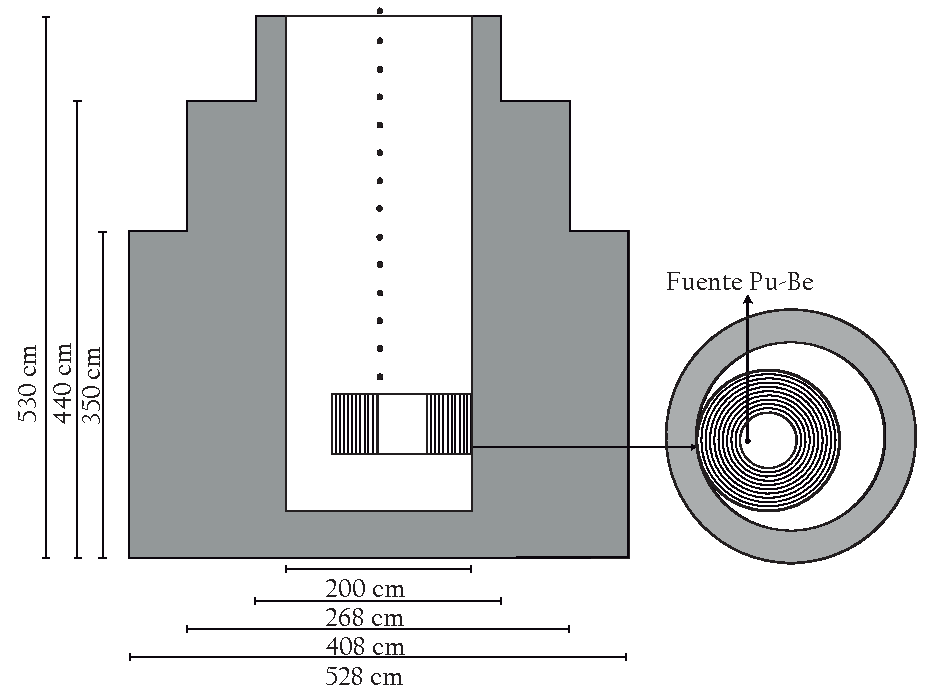
\includegraphics[scale=0.5]{Figuras/Art1Fig1.pdf}
    \caption{The caption should clearly explain the corresponding figure.}
    \label{fig:Example_Fig}
\end{figure}




\section{CONCLUSIONS.}

Conclusions should be clear and concise and can be enumerated. Their content should not substantially duplicate the abstract. They should express the final balance of the research or the application of knowledge on the topic. Discussion should revolve around the implications of the study and its relevance to the field of knowledge. It is suggested not to draw more conclusions than the results allow. This section typically mentions future work that can be carried out on the subject along with corresponding recommendations.

\noindent\footnotesize{{\bf Funding:} Please provide the funding entity here (if applicable).}\\

In addition to the acknowledgments, a conflict of interest declaration must be made.

\footnotesize{{\bf Declaration:} The authors declare no conflicts of interest.}



\section{ACKNOWLEDGEMENTS}

This section is necessary for research articles, where the author acknowledges individuals or institutions that assisted in their research. It may include grants and institutions that funded the research, commercial firms, official or private entities, professional associations, and collaborators. This section is optional for reflection articles. It is not a numbered section.

\textbf{Las referencias  se incluirán en el texto mediante números arábigos entre corchetes cuadrados  [ ], alineados con la escritura (formato IEEE), si son varias referencias juntas, se separarán con comas. Se enumerarán correlativamente
por orden de citación, apareciendo la lista al final del texto después de la sección de conclusiones o agradecimientos \cite{1},\cite{2}, \cite{3}.
}

\emph{
El estilo de referencias bibliográficas IEEE  es ampliamente utilizado en campos como la ingeniería, la electrónica y la informática. Aquí te presento cómo formatear las referencias bibliográficas en el estilo IEEE:}

\textbf{Libro:}

Apellido del autor, Inicial(es). (Año). Título del libro. Editor.

Ejemplo:

Smith, J. (2000). Introduction to Electrical Engineering. XYZ Publications.


\textbf{Capítulo de libro en una obra colectiva:}

Apellido del autor del capítulo, Inicial(es). (Año). "Título del capítulo". En Inicial(es) Apellido del editor (Ed.), Título del libro (páginas del capítulo). Editor.

Ejemplo:

Brown, R. (2015). "Advanced Circuits." En S. Johnson (Ed.), Electrical Engineering Handbook (pp. 112-135). ABC Publications.

\textbf{Artículo de revista:}

Apellido del autor, Inicial(es). (Año). "Título del artículo". Título de la revista, Volumen(Número), páginas.

Ejemplo:

Garcia, M. (2018). "An Analysis of Power Grids." IEEE Transactions on Power Systems, 30(2), 567-578.


\textbf{Conferencia o artículo de conferencia:}

Apellido del autor, Inicial(es). (Año, Mes de la conferencia). "Título del artículo". En Nombre de la conferencia (páginas). Editor.

Ejemplo:

Johnson, A. (2020, Julio). "Advancements in Robotics." En Proceedings of the International Robotics Conference (pp. 45-53). IEEE.

\textbf{
Documento en línea:}

Apellido del autor, Inicial(es). (Año). "Título del documento." Nombre del sitio web. [En línea]. Disponible en: URL. [Fecha de acceso: Día, Mes, Año].

Ejemplo:

Davis, S. (2019). "Introduction to Machine Learning." Machine Learning Central. [En línea]. Disponible en: https://www.example.com/ml-intro. [Fecha de acceso: 10 Septiembre 2023].

\textbf{Tesis:}

Apellido del autor, Inicial(es). (Año). "Título de la tesis." Tesis de Maestría/Doctorado, Nombre de la Universidad, Ciudad, País.

Ejemplo:

Chen, Q. (2017). "Design and Optimization of Communication Networks." Tesis de Doctorado, Universidad de California, Los Ángeles, EE. UU.
Recuerda que el formato exacto de las referencias puede variar según las directrices de la revista, conferencia o institución a la que envíes tu trabajo. Asegúrate de consultar las pautas específicas para garantizar que tus referencias cumplan con los requisitos del estilo IEEE que se solicitan.

\section{INTRODUCTION}

\justifying

All'interno di una comunicazione client-server, abbiamo che nei moderni browser può essere eseguito del contenuto dinamicamente, andando ad esempio a sfruttare quella che è la potenzialità offerta dai linguaggi di scripting come javascript. Ne consegue che all'interno dei browser possono essere memorizzate delle informazioni sensibili da proteggere dell'accesso di terzi non autorizzati, come ad esempio i cookie che possono contenere credenziali d'accesso e/o token d'autenticazione. A tale scopo sono state sviluppate delle policy di sicurezza per limitare (Same Origin Policy) e controllare (Content Security Policy) l'utilizzo e la gestione delle risorse all'interno delle pagine web riducendo i rischi di poter effettuare l'injection di codice malevolo. Tuttavia la policy CSP consegnata con una pagina web influisce solo sulle risorse della pagina stessa, non estendendosi automaticamente alle risorse incorporate nella pagina, come possono essere i tag html $<iframe>$. Questo comporta che anche nel caso in cui la pagina principale possa avere una politica CSP le regole non si applicano al contenuto all'interno degli iframe.
La diretta conseguenza è che, sfruttando l'origine in comune, si aprono le porte a diverse problematiche di sicurezza, consentendo l'esecuzione di codice arbitrario, raggirando quindi la Same Origin Policy (SOP), ma anche la possibilità di poter definire policy CSP differenti tra pagine importatrici e pagine importate tramite iframe, avendo in conclusione un'inconsistenza di regole definite nelle diverse policy. Verranno quindi individuate e replicate diverse casistiche per valutare se questa vulnerabilità è tutt'oggi una minaccia e valutare la possibilità di poter mitigare l'attuazione di tali scenari. 
\section{Background}
\justifying
In questa sezione andiamo a descrivere le caratteristiche che contraddistingue le \href{Origin}{origini}, la \href{chap:sameorigin}{Same-Origin-Policy (SOP)} e la \href{chap:contentsecpolicy}{Content-Security-Policy (CSP)}. 
\subsection{Origine, Dominio e Sub-Dominio}
\label{Origin}
In una comunicazione client-server il punto iniziale sta nel digitare un URL: 
\begin{center}
    \small\textit{http://www.main.com:80/dir/A.html}
\end{center}le risorse
Con il termine \textbf{Origin} si va ad identificare la terna: \textit{schema} (http), \textit{host} (main.com), \textit{porta} (81). Mentre l'ultima sezione, "/dir/A.html", va a definire la path del file indirizzato.\\
Per distinguere univocamente un indirizzo web si utilizzano i domini, nell'esempio precedente corrisponde all'host "main.com". A loro volta i domini possono essere suddivisi in sottodomini questi sono gerarchicamente inferiori e vengono utilizzati per definire in maniera più logica la struttura del sito web. Un esempio: 
\begin{center}
    \small\textit{http://www.sub.main.com}
\end{center}    

\subsection{Same Origin Policy}
\label{chap:sameorigin}
Come detto al paragrafo \ref{Origin}, una origine è formata dalla terna schema, host e porta. Una specifica utilizzata per proteggere i contenuti è la Same Origin Policy (SOP), questa consente ai programmatori di isolare i contenuti ritenuti non fidati \textit{(untrusted)}
provenienti da origini differenti. Questo meccanismo presente nei browser mantiene quindi al sicuro le informazioni relative ad un'origine (file .js, cookie, layout, ...) consentendone l'accesso solamente se l'origine di una richiesta è la stessa dei dati memorizzati. Senza l'implementazione di questa policy un utente malintenzionato potrebbe sfruttare i linguaggi di scripting per accedere a tali informazioni. \\
Suponendo di avere il seguente URL: 
\begin{center}
    \small\textit{http://main.com/dir/A.html}
\end{center}
Avremo come origine \textit{http://main.com}, se la porta non è specificata sarà la porta di default dello schema, nel caso dell'Http, la porta 80. Di seguito nella tabella \ref{tab:SOPTABLE1} possiamo osservare varie casistiche che descrivono il comportamento della Same Origin Policy. 

\begin{table}[h] % Utilizzo di [h] per posizionare la tabella "qui"
\centering % Centra la tabella
% Inizia la tabella
\begin{tabular}{|c|c|} % specifica il formato delle colonne (centrate, con linea verticale tra di loro)
\hline % linea orizzontale superiore della tabella
\rowcolor{gray!30} % Colora l'intera riga con il 50% del grigio
URL & Violazione SOP  \\ % contenuto della tabella
\hline % linea orizzontale sotto l'intestazione delle colonne
http://main.com/\textbf{dir2}/A.html & No \\
http://main.com/\textbf{dir/dir2}/A.html & No \\
\textbf{https}://main.com/dir/A.html & Si, schema differente \\
http://main.com:\textbf{81}/dir/A.html & Si, porta differente \\
http://\textbf{sub.}main.com/dir/A.html & Si, host differente \\
\hline % linea orizzontale inferiore della tabella
\end{tabular}
\caption{Comparazioni violazioni SOP} % Didascalia della tabella
\label{tab:SOPTABLE1} % Etichetta per referenziare la tabella
\end{table}

\subsection{Content Security Policy}
\label{chap:contentsecpolicy}
Con la Content-Security-Policy, si sposta l'attenzione al controllo, lato client, delle risorse che possono essere caricate ed eseguite all'interno di una pagina nel browser. Ad oggi CSP è supportato da tutti i principali browser \cite{3}.\\
La Content-Security-Policy è un ulteriore livello di sicurezza il cui obiettivo primario è quello di mitigare gli attacchi Cross-Site-Scripting (XSS). Consente agli sviluppatori di specificare e controllare quale risorsa client-side possa essere caricata ed eseguita dai browser. In questo modo si previene l'accesso al contenuto dalle risorse considerate \textit{untrusted}.\\
Per definire una politica CSP si può procedere configurando il web-server definito gli Header response HTTP oppure specificando le direttive nei tag \textit{$<meta>$} dell'HTML come nell'esempio in Listing \ref{meta-csp-def-ex} 

\begin{lstlisting}[
    language=HTML,
    caption=Esempio definizione CSP nel tag meta,
    label=meta-csp-def-ex,
    backgroundcolor=\color{codegray}, % Colore di sfondo
    frame=tb, % Visualizzazione del bordo intorno al codice
    frameround=ffff, % Stile del bordo
    framesep=15pt, % Spazio tra il bordo e il contenuto
    xleftmargin=15pt, % Margine sinistro
    xrightmargin=15pt, % Margine destro
    keywordstyle=\color{tagblue}\bfseries,
    morekeywords={html, head, title, body, h1, p}, % Aggiunta di nuove parole chiave (tag HTML)
    basicstyle=\fontsize{8}{9}\selectfont\ttfamily, % Modifica del font e della dimensione del carattere 
]
<html>
<head>
    <meta http-equiv ="Content-Security-Policy"
          content ="default-src 'self'; 
                    img-src https://*;
                    script-src 'none';">
</head>
</html>
\end{lstlisting}
Le direttive che si possono definire sono molteplici in tabella \ref{tab:directives} vengono elencate le più comuni.
\begin{table}[h] % Utilizzo di [h] per posizionare la tabella "qui"
\centering % Centra la tabella
 {\fontsize{9}{10}\selectfont % Imposta la dimensione del testo 
    \begin{tabular}{|c|c|}
    \hline % linea orizzontale superiore della tabella
    \rowcolor{gray!30} % Colora l'intera riga con il 50% del grigio
        \textbf{Directive} & \textbf{Controlled content} \\
        \hline
        \texttt{script-src} & Scripts \\
        \texttt{default-src} & All resources (fallback) \\
        \texttt{style-src} & Stylesheets \\
        \texttt{img-src} & Images \\
        \texttt{font-src} & Fonts \\
        \texttt{connect-src} & XMLHttpRequest, WebSocket, or EventSource \\
        \texttt{object-src} & Plug-in formats (object, embed) \\
        \texttt{report-uri} & URL where to report CSP violations \\
        \texttt{media-src} & Media (audio, video) \\
        \texttt{child-src} & Documents (frames), [Shared] Workers \\
        \texttt{frame-ancestors} & Embedding context \\
        \hline
    \end{tabular}
    }
\caption{Direttive CSP più comuni} % Didascalia della tabella
\label{tab:directives} % Etichetta per referenziare la tabella
\end{table}
Entrando più nello specifico abbiamo che la direttiva \textit{script-src} è la più utilizzata, questa definisce da quali origini è consentito caricare e eseguire script all'interno di una pagina web andando a definire uno o più attributi come: 
\begin{itemize}
    \item \textit{'self':} consente l'esecuzione di script dalla stessa origine;
    \item \textit{'http://example.com':} consente l'esecuzione di script dall'origine specificata;
    \item \textit{'none':} direttiva molto restrittiva che non consente l'esecuzione di alcuna tipologia di script; 
\end{itemize}
Quando si va a definire la direttiva \textit{scritp-src}, oltre a non poter importare file o snippet di scripting untrusted, non sarà possibile eseguire gli script-inline ovvero script eseguiti direttamente nel codice HTML attraverso il tag $<script>$ oppure gli handlers 'onclick' ed 'onload'. Questa caratteristica può essere rimossa andando a specificare l'attributo 'unsafe-inline'. Tuttavia utilizzarlo è considerato un comportamento non sicuro in quanto qualsiasi script può essere introdotto ed eseguito. 
\subsubsection{CSP e XSS Attack}
La Content-Security-Policy va quindi a mitigare la possibilità di riuscita di attacchi di tipo Cross-Site-Scripting (XSS). In questa tipologia di attacchi un utente malintenzionato mira a sfruttare una vulnerabilità all'interno di una pagina web per iniettare e far eseguire degli script dannosi. Dando la possibilità agli sviluppatori di poter definire tramite CSP quali risorse possono essere eseguite all'interno della pagina web e quindi potendo controllare le origini che possono caricare script, immagini e style si riduce di molto la potenziale riuscita di injection di codice malevolo. 

%\subsection{Vulnerabilità}

\section{Motivazioni}
\justifying 
Definita una policy CSP all'interno di una pagina Web questa si applica solamente alle risorse inerenti la pagina stessa, di conseguenza non viene estesa ad elementi incorporati all'interno del codice come iframe. Nello specifico considerando una web-page nella quale si utilizzano iframe ed \underline{appartenenti alla stessa origine}, si può incorrere nelle seguenti casistiche:\\
\textbf{- Solamente la pagina importatrice dell'iframe ha definita una policy CSP:} In questo caso il codice contenuto nell'iframe raggirerà sia SOP che la policy CSP. Un attacco XSS è possibile in quando il codice contenuto nell'iframe è potenzialmente vulnerabile e per via dell'inconsistenza tra SOP e CSP questa vulnerabilità si estenderà al codice della pagina potendo accedere al codice della pagina principale.\\
\textbf{- Solamente il codice all'interno dell'iframe ha definita una policy CSP:} Questo comporta che la pagina principale sia vulnerabile ad eventuali attacchi XSS ed importando un iframe in cui è definita una policy CSP provenendo dalla stessa l'eventuale codice malevolo può dalla pagina principale accedere al codice dell'iframe. \\

Un ulteriore caso è quello che riguarda la comunicazione tra la pagina principale (main.com) ed una pagina appartenente ad un suo sotto-dominio (sub.main.com). Benché condividano lo stesso dominio di alto livello, SOP valuta queste due origini differenti andando a bloccarne la comunicazione. Tuttavia quello che può accadere è che utilizzando la direttiva \textit{document.domain} la pagina importata (sub.main.com) può cambiare il suo dominio, rilassandolo al dominio di primo livello diventando di fatto "main.com". in questo modo sia nel caso in cui la pagina principale o la pagina all'interno dell'iframe non abbiano una policy CSP implementata, oppure nel caso abbiano due policy CSP diverse, è possibile raggirare SOP rendendo possibile  gli attacchi precedentemente descritti. 
%Scoperto che doc.domain è deprecato va nei risultati ;D

\section{Lavori correlati}
Il lavoro del 2017 di Dolière et al. \cite{1} pone l'attenzione sull'inconsistenza tra la CSP e la SOP nell'utilizzo di strutture HTML $<iframe>$. Alti lavori hanno studiato la Content-Security-Policy individuando problemi legati alla mancanza di aggiornamento regolare delle direttive \cite{5}. Mentre altri lavori si sono concentrati sull'individuare bug all'interno delle direttive CSP *inserisc i citazione se lo metti*
\section{Lavori correlati}
\justifying
Il lavoro del 2017 di Dolière et al. \cite{1} pone l'attenzione sull'inconsistenza tra la CSP e la SOP nell'utilizzo di strutture HTML $<iframe>$. Alti lavori hanno studiato la Content-Security-Policy individuando problemi legati alla mancanza di aggiornamento regolare delle direttive \cite{4}. 
\section{OBIETTIVI}
\label{chap:obiettivi}
\justifying
Gli obiettivi principali di questo lavoro si concentrano sull'andare a: 
\begin{center}
    \textbf{$OB_1$}: \textbf{replicare gli attacchi proposti} dal lavoro \cite{1}. Nello specifico i test di replica saranno eseguiti su un ambiente di sviluppo costituito da Google Chrome versione 51.0.2704 eseguito su una macchina virtuale con sistema operativo Linux Ubuntu 16.04.\\
    \textbf{$OB_2$}: successivamente andare a \textbf{valutare se gli attacchi siano ancora replicabili su un ambiente aggiornato a Gennaio 2024} ed a seconda dei risultati ottenuti individuare le mitigazioni attuate o possibili.\\
    
\end{center}
Come obiettivo finale, si vuole rispondere alla domanda sull'\textbf{esistenza di una soluzione/mitigazione in grado di garantire la costruzione di siti web sempre sicuri} contro questa vulnerabilità e se tale soluzione venga effettivamente implementata o meno.
\section{METODOLOGIA E PRODOTTO FINALE}
\justifying
Come primo step per la replicazione degli attacchi, si procederà andando ad individuare tutte le casistiche possibili. Successivamente bisognerà creare una environment virtualizzato che risponda alle specifiche descritte nel lavoro \cite{1}. 
Per la creazione dei web server e per la specifica dei differenti domini necessari alla sperimentazione si userà la tecnologia \href{https://www.docker.com/}{Docker}. Il codice sviluppato andrà ad effettuare l'injection e raggirando le policy accederà a delle specifiche variabili. Si procederà infine alla ricerca di eventuali strategie di mitigazioni valutando la possibilità di poterle attuare.

\subsection{Prodotto finale}
Alla fine della sperimentazione si presenteranno i risultati relativi la riuscita o meno della replicazione degli attacchi ed i dati relativi la possibilità di attuare o meno delle mitigazioni per la tipologia d'attacco in esame. Il codice sviluppato sarà disponibile all'interno della repository GitHub\footnote{\href{https://github.com/AndreaDagg/CSP-vulnerability-due-to-SOP}{https://github.com/AndreaDagg/CSP-vulnerability-due-to-SOP}}. In conclusione verrà redatto un documento che conterrà tutte le discussioni sugli obiettivi e le tecnologie utilizzate nel dettaglio per il raggiungimento dei risultati finali.






%%%%%%%%%%%%%%%%%%%%%%%%%%%%%%%%% BIBLIOGRAFIA %%%%%%%%%%%%%%%%%%%%%%%%%%%%%%%%%%%%%%%%%%%%%%
\newpage
\vspace{14em}
\begin{thebibliography}{4}

\bibitem{1}
\href{https://dl.acm.org/doi/10.1145/3038912.3052634#sec-comments}{Some, Doli\`{e}re Francis and Bielova, Nataliia and Rezk, Tamara (2017)}\\
On the Content Security Policy Violations Due to the Same-Origin Policy.
\textit{Proceedings of the 26th International Conference on World Wide Web}, 877--886.\\
\small{\url{https://dl.acm.org/doi/10.1145/3038912.3052634#sec-comments}}\\
\bibitem{2}
\href{https://developer.mozilla.org/en-US/docs/Web/Security/Same-origin_policy}{MDN Web docs - Same-origin policy}\\
\small{\url{https://developer.mozilla.org/en-US/docs/Web/Security/Same-origin_policy}}\\
\bibitem{3}
\href{https://developer.mozilla.org/en-US/docs/Web/HTTP/CSP}{MDN Web docs - Content Security Policy (CSP)}\\
\small{\url{https://developer.mozilla.org/en-US/docs/Web/HTTP/CSP#browser_compatibility}}\\
\bibitem{4}
\href{https://dl.acm.org/doi/abs/10.1145/3149408}{Calzavara, Stefano and Rabitti, Alvise and Bugliesi, Michele}\\
Semantics-Based Analysis of Content Security Policy Deployment,
\textit{anno = {2018}}\\
\url{https://dl.acm.org/doi/abs/10.1145/3149408}

\end{thebibliography}

\end{document}